% This is file JFM2esam.tex
% first release v1.0, 20th October 1996
%       release v1.01, 29th October 1996
%       release v1.1, 25th June 1997
%       release v2.0, 27th July 2004
%       release v3.0, 16th July 2014
%   (based on JFMsampl.tex v1.3 for LaTeX2.09)
% Copyright (C) 1996, 1997, 2014 Cambridge University Press

\NeedsTeXFormat{LaTeX2e}

\documentclass{jfm}
%\documentclass[referee]{jfm} %for double spaced output for submission

% See if the author has AMS Euler fonts installed: If they have, attempt
% to use the 'upmath' package to provide upright math.
\usepackage[english]{babel}
\usepackage{graphicx}
\usepackage{latexsym}
\usepackage{natbib}
\usepackage{rotate}
\usepackage{epstopdf}
\usepackage{pstricks}
\usepackage{amsmath}
\usepackage{url}
\newtheorem{lemma}{Lemma}
\usepackage{mathrsfs}  
\usepackage{latexsym}
\newtheorem{corollary}{Corollary}

\newcommand\be{\begin{equation}}
\newcommand\ee{\end{equation}}
\newcommand\bea{\begin{eqnarray}}
\newcommand\eea{\end{eqnarray}}
\newcommand\DP[2]{\frac{\p #1}{\p #2}}


%\pubyear{2012}
%\volume{}
%\pagerange{}
\date{\today}
%\setcounter{page}{1}

\shorttitle{Acoustic forcing of a laminar viscous jet through a thick circular aperture}
\shortauthor{D. Fabre, R. Longobardi, P. Bonnefis and P. Luchini}

\title{Acoustic forcing of a laminar viscous jet through a circular aperture in a thick plate : Impedance calculations and instability criteria}

\author{David Fabre\aff{1}
  \corresp{\email{david.fabre@imft.fr}},
  Raffaele Longobardi\aff{1,2},
  Paul Bonnefis\aff{1}
 \and Paolo Luchini\aff{2}}
\affiliation{\aff{1}Institut de M\'ecanique des Fluides de Toulouse, IMFT, Universit\'e de Toulouse, CNRS; All\'ee Camille Soula, 31400 Toulouse, France
\aff{2}DIIN (Dipartimento di Ingegneria Industriale); Universit\'a degli Studi di Salerno; Via Giovanni Paolo II, 84084 Fisciano (SA), Italy}

\begin{document}


\maketitle

\begin{abstract}
THIS IS THE ABSTRACT OF PART I !!!!!
The unsteady flow through a circular aperture in a thin plate subjected to harmonic forcing (for instance under the effect of an incident acoustic wave) is a classical problem first considered by Howe  ({\em Proc. R. Soc. London. A}, vol. 366, 1979, pp. $205-223$), using an inviscid model. The purpose of this work is to reconsider this problem through a  numerical resolution of the incompressible linearized Navier$-$Stokes equations (LNSE) in the range $Re = [100,3000]$. We first compute a steady base flow which allows us to describe the {\em vena contracta} phenomenon in accordance with experiments. We then solve a linear problem allowing to characterize both the spatial amplification of perturbations and the impedance (or equivalently the Rayleigh conductivity), which is a key quantity to investigate the response of the jet to acoustic forcing. Since the linear perturbation is characterized by a strong spatial amplification, the numerical resolution requires an original method based on the complex mapping of the axial coordinate in order to enlarge the range of Reynolds number investigated. 
The results show that the impedances computed with $Re\gtrsim 1500$ collapse onto a single curve, indicating that a large-Reynolds number asymptotic regime is effectively reached. However, expressing the results in terms of conductivity leads to substantial deviation with respect to the Howe model.
%The predictions for the Rayleigh conductivity are in good qualitative agreement with the model of Howe in the range of high Reynolds numbers. 
Finally, we investigate the case of finite amplitude perturbations through direct numerical simulations (DNS). We show that the impedance predicted by the linear approach remains 
valid for amplitudes up to order $\textit{O}(10^{-1})$, despite the fact that the spatial evolution of perturbations in the jet is strongly nonlinear.
\end{abstract}


\begin{keywords}

\end{keywords}

\section{Introduction}
%change the first sentence
The problem of the flow passing through a circular aperture in a plate is encountered in many practical applications, as for example fuel injectors, cooling system for gas turbines or wind instruments. 
When subjected to harmonic forcing, for instance under the effect of an incident acoustic wave, the vortex sheet formed at the rim of the aperture becomes periodically modulated and acts as a spatial amplifier of Kelvin-Helmholtz instability, reorganizing the jet into an array of vortex rings. This feature is an essential part of the sound production mechanism in situations where the jet subsequently passes through a second aperture, a configuration known as ``hole-tone'' and encountered for instance in tea kettles \citep{henrywood2013aeroacoustics} and birdcalls \citep{fabrea2014application}. The generation of vorticity is also an efficient mechanism to dissipate the acoustic energy. As a consequence, the use of multiply perforated plates traversed by a mean flow (or bias flow) is widely used as a sound attenuator device in many industrial applications, such as combustion systems.

The unsteady, periodic flow through a circular hole in a zero-thickness plate was initially solved by \citet{rayleigh1945theory} using inviscid, potential theory. The key result of his solution is the proportionality between the net pressure force felt from both sides of the hole and
the acceleration of the fluid, so that the whole situation can be modeled by assuming that there is a rigid plug of fluid, with area $A_h=\upi R_{h}^2$ and equivalent length $\ell_{eff}$, oscillating across the aperture, where $R_h$ is the radius of the hole.

The case where the flow has a mean component (or bias flow) in addition to the oscillating component was considered by \citet{howe1979theory}. He introduced a key quantity, the Rayleigh conductivity $K_R$, defined as the ratio of the acceleration of the fluid particules located within the aperture to the net force exerted on it. The real part of the conductivity generalizes the concept of equivalent length $\ell_{eff}$ previously introduced by Rayleigh, while its imaginary part is directly proportional to the flux of energy transferred from the imposed oscillatory flow to the jet. Under the hypothesis of high Reynolds number, low Mach number, and assuming that the oscillating flow is of small amplitude with respect to the mean flow, Howe derived an theoretical model describing the vorticity shed at the rim of the aperture and predicting the real and imaginary parts of the conductivity by analytical formulas. However, despite its mathematical rigour, the Howe's model starts from very simplified and limitating hypothesis regarding the shape and the location of the vortex sheet and its convective velocity. Recently, \citet{fabre2018} reviewed the Howe's problem using the Linearized Navier$-$Stokes equations in order to take into accout the effect of the viscosity and the exact shape of the vortex sheet. They show that for $Re \gtrsim 1500$, results are quite independent from the Reynolds number but they result to be quite different from the Howe's ones, above all for intermediate fequencies. 

UNTIL HERE IS THE FIRST PART OF THE PART I INTRO: TO MODIFY.

A similar, but more realistic situation is the one in which the flow passes through a hole in a thick plate. Many analytical and semi$-$empirical models can be found in the dedicated literature in order to take into account the effect of the hole's length. 
\citet{bellucci2004use} found out a correction to Howe's model using a momentum balance for a one$-$dimensional flow crossing the hole. \citet{jing2000effect}, instead, improved Bellucci's model used boundary elements method and experimental data in order to interpolate the shape of the vortex sheet.
In order to improve the shape of the vortex sheet, recently \citet{yang2016semi} developed a semi$-$analytical model based on a free space Green formula, showing the inportance to capture the actual shape of the vortex noise. However, they considered the potential inviscid flow combined with a Kutta condition at the leading edge \citep{crighton1985kutta} in order to remove the singularity.
The literature cited until here does not consider the effect of the viscosity on such kind of flow configurations. \citet{eldredge2007numerical} performed incompressible Large Eddy Simulations (LES) to characterize the linear acoustic response of a turbulent flow tangential to both sides of a multi$-$perforated liner. They found a good agreement with the inviscid model by \citet{jing2000effect}, but only when \emph{ad$-$hoc} parameters of this model are selected in order to take into account the thickness of the hole, demonstrating that this model is not robust. \citet{su2015measurements} investigated the effect of linear acoustic oscillations of short and long holes. They used the Unsteady Navier$-$Stokes Equations (URANS) for a compressible low$-$Mach number flow and they found very good agreement with their own experiments but not with the inviscid model by \citet{jing2000effect}, in particular for very long holes respect to their diameters. If the viscosity is not considered, the acoustic boundary layer is not solved, leading to an excessive amount of vorticity and consequently to an overprediction of the whistling properties of the hole, as discussed by \citet{kierkegaard2012simulations}.
%%%%OBJECTIVES
Analyzing the current literature, it seems that the shape of the vortex sheet and the viscosity play a crucial role into the prediction of the acoustic properties of such kind of flow configurations. As far as the viscosity, however, the above cited authors calculated the impedance of circular holes in a turbulent regime (modelling the turbulence with LES or RANS techniques). Moreover, they didn't characterize the effect of the Reynolds number variation.
In this paper, we consider the oscillating ``laminar'' flow passing through a circular aperture in a thick plate, in order to take into accout the effect of both the hole length, the shape of the vortex sheet (with a precise description of the {\em vena contracta} phenomenon) and the variation of the Reynolds number (viscosity). In order to pursue this objectives, following the previous work by \citet{fabre2018} about the zero$-$thickness hole, we use the Linearized Navier$-$Stokes Equations (LNSE). Moreover, as demonstrated by the authors in this previous work, the computation of such kind of flow is notoriously difficult for two reasons. First, the base flow is characterized by a shear layer which remains very steep far away from the aperture, leading to the necessity of a very long computational domain in the axial direction. Secondly, the jet is strongly convectively unstable due to the Kelvin-Helmholtz instability, and it is difficult to design a method capturing both the coupling between the flow rate and the pressure jump, which is relevant to characterize the acoustic properties of the hole, and the spatial growth of perturbations in the axial direction, which can reach huge levels as far as the Reynolds number increases. Following the authors, we adopt the complex mapping of the axial coordinate $x$ in order to obtain suitable results up to $\Rey = 10^4$.\\

Finally, the main objectives of this paper can be summarized as follows.

\begin{itemize}
\item[(i)] First, we describe the base flow characteristics, focusing our attenction on the {\em vena contracta} phenomenon and the intensity of the recirculation bubble, varying the length of the hole.
 
 \item[(ii)]  Secondly, we investigate the linear response of the jet to harmonic forcing. We compute the impedance varying the length of the hole. We show that because of the thickness of the hole different mechanisms take place and the jet acts like a sound generator rather than a sound dampers. We show that the combined analysis of its real and imaginary parts gives important information about the stability of such kind of flow and the possibility of self$-$sustained oscillation processes \citep{howe1997influence}, which are responsable of the whistling emission. 

\item [(iii)] Finally, We discuss the spatial structure of the forced problem.
\end{itemize}


 
 \section{Problem definition}
%The Howe's problem has been reviewed already in part I...we could talk about the end correction models.
\subsection{Problem definition}

\begin{figure}
$$
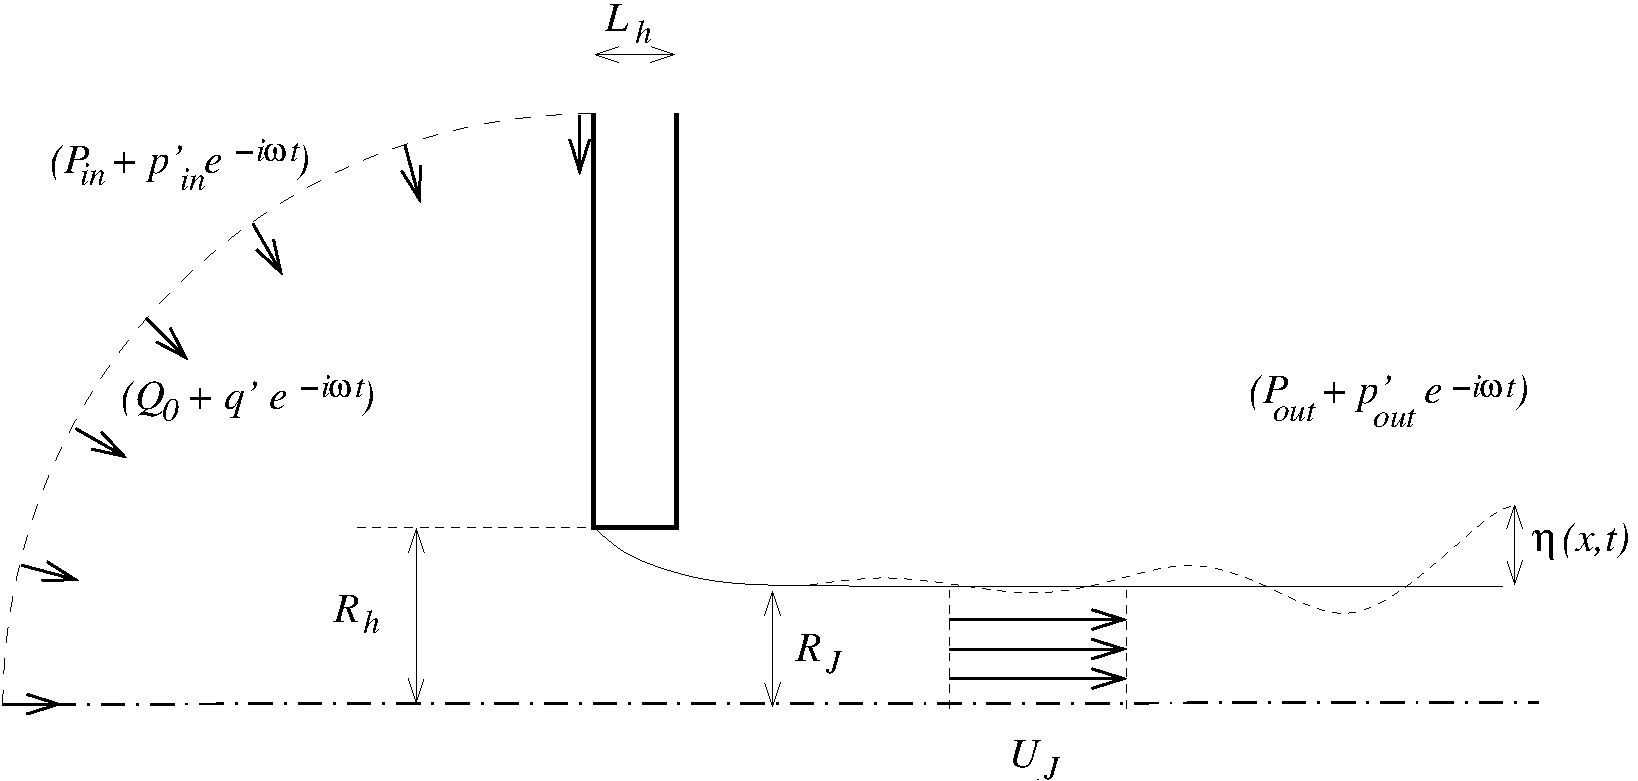
\includegraphics[width = .8 \linewidth]{FIGURES/SketchJetNV.pdf}
$$
\caption{Oscillating flow through a circular hole : inviscid modeling} 
\label{fig:Problem+Model}
\end{figure}


The situation considered here is the flow of an incompressible fluid of density $\rho$ and viscosity $\nu$ through a circular hole or radius $R_{hole}$ and area $S_{hole}= \pi R_{hole}^2$ inside a planar plate of thickness $H_{hole}$, connecting an inner domain and an outer domain. We note $Q$ the volumic flux through the hole, defined as follows :

$$
Q = \int_{\cal S} {\bf u}\cdot {\bf n} d S,
$$
where $\cal S$ is any surface traversed by the flow, and $\bf n$ the normal vector at this surface.

We also note $p_{in}$ and $p_{out}$ the pressure levels far away from the hole, in the upstream and downstream domain respectively.

\subsection{Steady flow}

Consider, first, the steady flow. We note $Q_0$, $P_{in}$ and $P_{out}$ the values of the volumic flux, upstream and downstream pressure.

In the inviscid case, a classical model was proposed by Levi-Civita and Prandtl. The model consists of a vortex sheet formed at the hole, surrounding the jet (see figure 1). After several diameters, the jet becomes parallel, but with a radius $R_J$ smaller than that of the hole. We classically call the ratio of surfaces $\alpha = (\pi R_J^2)/(\pi R_h)$ The {\em venna contracta} coefficient. This coefficient is classically associated to the pressure loss across the aperture. Assuming a constant velocity $U_J$ inside the jet, the conservation of flux through the hole leads to 
$Q = \pi R_J^2 U_J = \pi R_h^2 U_M^2$. Applying the Bernoulli theorem along streamlines passing through the hole thus leads to 
\be
[P_{in}-P_{out}] = \frac{\rho U_J^2}{2} = \frac{\alpha^2  \rho U_M^2}{2}
\label{eq:alpha}
\ee
%Therefore, the coefficient $\alpha$ is directly related to the pressure loss through the hole. 
Theoretical calculations by Prandtl and Levi Civita provide the value $\alpha = 0.5$ while experiments indicate typical values in the range $0.61< \alpha< 6.64$ for Large-Reynolds number flows. The global approach used in the sequel will allow to compute rigorously this parameter for arbitrary values of the Reynolds number, assuming laminar flow.

%From a practical point of view, the most important quantity associated to the base flow is the pressure drop $(P_in - P_out)$ and its relation with the volumic flux. This relationship is classically expressed through the so-called {\em venna contracta} coefficient $\alpha$. 

%$Q = S_h U_M = S_J U_J$ 

%Where  $\alpha = S_J/S_h$ is the venna contracta coefficient.


\subsection{Unsteady flow}

We now reconsider the relationship between the pressure jump and the flow rate in the unsteady case, assuming a harmonic time dependance with frequency $\omega$. Hence, upstream and downstream pressure levels and the flow rate are 

$$
p_{in} = P_{in} + p'_{in} e^{-i \omega t} ; \quad p_{out} = P_{out} + p'_{out} e^{-i \omega t} ; \quad Q = Q_0 + q' e^{-i \omega t}.
$$

It is convenient to introduce the Strouhal number $\Omega$ 

$$ 
\Omega = \frac{\omega R}{U_M}.
$$



We are still interested in the relationship between pressure jump and flow rate. This relationship can be characterized by the {\em impedance} of the apperture, defined as 
$$
Z_{app} = \frac{[p_{in}'-  p_{out}']}{q'}.
$$
An alternative definition was introduced by Rayleigh, who defined the {\em conductivity} $K$ of the aperture as follows :

$$
K = \frac{-i \omega \rho q'}{[p_{in}'-  p_{out}']} \equiv \frac{- i \omega \rho}{Z_{app}}  
$$

The advantage of this definition is that it has the physical dimension of a length, and a simple physical interpretation. Namely, one can recognize in this definition a proportionality between the acceleration of the fluid through the aperture and the net force exerted on it. Indeed, this proportionality can be recovered by assuming that the fluid in the vicinity of the hole behaves as a simple solid plug with mass $\rho \pi R_h^2 \ell_{eff}$ oscillating across the hole. Hence, when it is real, $K$ is directly related to the {\em equivalent lengh} of fluid
through $K = A/\ell_{eff}$ with $A = \pi R_h^2$ the area of the aperture. 
%a quantity which appears, for instance, in the classical modeling of the Helmholtz resonator. 
For a hole of zero thickness, Rayleigh gives the theoretical value $\ell_{eff} = 2 R/ \pi$, hence $K = 2R$
while for a very thick plate ($L_h\gg R_h$) one has $\ell_{eff} = L_h + 1.28 R_h$  (to be checked, and give references). 


The problem of Rayleigh was reconsidered by Howe, in presence of a base flow, leading to a prediction for the conductivity as function of the Strouhal number. The derivation is extremely technical and not reproduced here. The final result amounts to :
$$
K = 2R ( \gamma - i \delta)
$$
with
\be
\gamma = \frac{
I_1(\Omega^*)^2[1+1/\Omega^*]+(4/\pi^2) e^{2\Omega^*}\cosh(\Omega^*) K_1(\Omega^*)^2[\cosh(\Omega^*)-\sinh(\Omega^*)/\Omega^*]
}
{
I_1(\Omega^*)^2+(4/\pi^2) e^{2\Omega^*}\cosh^2(\Omega^*) K_1(\Omega^*)^2
}
\label{eq:gammaHowe}
\ee

\be
\delta = 
\frac{
(2/\pi \Omega^*) I_1(\Omega^*) K_1(\Omega^*)e^{2\Omega^*}
}
{
I_1(\Omega^*)^2+(4/\pi^2) e^{2\Omega^*}\cosh^2(\Omega^*) K_1(\Omega^*)^2
}
\label{eq:deltaHowe}
\ee

Note that in the calculation of Howe, the Strouhal number is defined as $\Omega^* = \omega R/U$ where $U$ is the velocity of convection of the vorticity along the vortex sheet. Howe argues that $U= U_J/2$, in accordance with the classical modeling of the Kelvin-Helmholtz instability.
Hence the relationship with the Strouhal number used in the present paper is $\Omega^* = \Omega/(2 \alpha)$, and the two definitions are equivalent if $\alpha = 1/2$.

\subsection{Energy flux and instability criteria}


An important property of the Rayleigh conductivity is that it is directly related to the energy flux transmitted to the flow. This was demonstrated by Howe, leading to the following formula :

\be
\left< \Pi_{jet} \right>  = \frac{ |p'_{in}|^2 R \delta}{\rho_0 \omega} 
\quad 
\left( \, = \frac{\rho_0 \omega R \delta | q' |^2 }{|K^2|} \, \right) 
\label{eq:Pienergy}
\ee

\be
\left< \Pi_{jet} \right>  = \left< (p'_{in}-p'_{out}) q'  \right> 
\left( \, = \frac{Z_R | q' |^2 }{2} \, \right) 
\label{eq:Pienergy}
\ee

In the inviscid model of Howe, the term $\delta$ given by Eq. (\ref{eq:deltaHowe}) is always positive, meaning that 
exciting the jet at a given frequency necessitates the provision of energy by an outer system. 
Conversely, a negative $\delta$ means that oscillations of the jet can supply to an outer system, which can be for instance an acoustic resonator. 

IMPORTANT: TALK ABOUT THE NYQUIST CRITERIA!!!!



\section{The viscous problem : analysis and numerical method}


\subsection{Parameters and general equations}



The dimensions of the inner and outer domains are assumed to be large compared to the dimensions of the hole, so the only physically meaningful parameter is the aspect ratio of the hole defined as follows : 

$$
\beta = \frac{ L_{hole}}{2 R_{hole}}.
$$

Taking the diameter $2 R_{hole} $ as a length scale and the average velocity through the hole  $U_M/\pi R_{hole}^2$  as a velocity scale, we can define a Reynolds number and an aspect ratio :

$$ 
Re = \frac{ 2 R_{hole} U_M}{\nu} \equiv \frac{2 Q }{ \pi R_{hole} \nu} ; \quad
$$ 

The problem is governed by the Navier-Stokes equations which are written in the following form
  
\be
\DP{ }{t} \left[\begin{array}{c} {\bf u} \\ 0 \end{array} \right] = 
{\cal NS} \left[\begin{array}{c} {\bf u} \\ p \end{array} \right] =
 \left[\begin{array}{c}
- {\bf u} \cdot \nabla {\bf u} - \nabla p + \nu \Delta {\bf u} \\
 \nabla \cdot {\bf u} 
\end{array} \right] 
\label{eq:NS}
\ee 

The flow is further decomposed into a base flow $[{\bf u_0};p_0]$ associated with the mean flux $Q_0$ and a small-amplitude perturbation  $[{\bf u}';p']e^{-i \omega t}$ associated with the oscillating flux $q' e^{-i \omega t}$.
The base flow obeys the steady Navier-Stokes equations ${\cal NS} [{\bf u_0};p_0] = 0$
and the perturbations obeys the linear equation $- i \omega [{\bf u}';0] = {\cal L}_0 [{\bf u}';p']$ where ${\cal L}_0$
is the linearized Navier-Stokes operator about the base flow, defined as follows: 
\be
{\cal L}_0 \left[\begin{array}{c} {\bf u}' \\ p' \end{array} \right] =
 \left[\begin{array}{c}
- \left( {\bf u}_0 \cdot \nabla {\bf u}' +{\bf u}' \cdot \nabla {\bf u}_0 \right) - \nabla p' + \nu \Delta {\bf u}' \\
 \nabla \cdot {\bf u}' 
\end{array} \right] 
\label{eq:NS}
\ee 

 The detailed expression of these operators will be given below. The flow obviously verifies no-slip conditions ${\bf u} = {\bf 0}$ on the wall (noted $\Gamma_w$),  and symmetry conditions at the axis (noted $\Gamma_{ax}$). The treatment of the geometry and boundary conditions in the upstream and downstream domain require special attention and are detailed bellow.

\subsection{Upstream domain}

As sketched in figure 1, the upstream domain is expected to originate from an upstream container of large dimension, and sufficiently far away from the hole the flow is assumed to be radially convergent. However, in the numerical implementation, it is required to specify a given geometry for this upstream domain. Here, we have chosen to assume that the upstream region is a closed cavity of rectangular cross-section, with radius $R_{cav}$ and length $L_{cav}$. The volumic flux condition is imposed by assuming that both the base-flow and the perturbation velocities are constant along the bottom of the cavity, noted $\Gamma_{in}$

\be
 {\bf u}_0 = - Q_0/S_{cav} {\vec n} ; \quad {\bf u'} = - q'/S_{cav} {\vec n} \quad {\mbox at } \Gamma_{in}
\ee
where $S_{cav}= \pi R_{cav}^2$ is the area of the bottom wall and ${\bf n}$ is the outward normal vector.
The pressure levels $P_{in}$ and $p'_{in}$, which are required for the calculation of the mean pressure loss and the conductivity, are computed by averaging along the inlet boundary :
\be
 {P}_{in} = 1/S_{cav} \int_{\Gamma_{in}} P_0 2 \pi r dr ; \quad
  {p'}_{in} = 1/S_{cav} \int_{\Gamma_{in}} p' 2 \pi r dr.
\ee
It was verified that if the dimensions of the cavity are large enough, the pressure is effectively nearly constant along the inlet boundary $\Gamma_{in}$.

At the lateral wall of the cavity, noted $\Gamma_{lat}$, the physically relevant condition should be a no-slip condition. However, as the location of this wall is not really relevant, and in order to avoid the development of a boundary layer, 
we preferred to impose a stress-free condition, namely  
\be
 {\bf u} \cdot {\bf n} = 0 ; \quad \DP{({\bf u} \cdot {\bf x})}{r} = 0 \quad \mbox{  at  } \Gamma_{lat},
 \ee
which applies for both the base flow and the perturbation.

In the sequel we set the dimensions of the upstream cavity as $L_{cav} = R_{cav} = 10 R_{hole}$,
and verified that these values are large enough for the results to be insensible to these parameters.

\subsection{Downstream domain : boundary conditions and change of coordinates}

The treatment of the outlet conditions is a delicate point here, as the structure of both the base flow and the perturbation lead to some difficulties, especially when the Reynolds number becomes large. These difficulties led us to use an original method which consists of using a change of variables from a computational domain defined with $[X,R]$ coordinates to the physical domain with $[x,r]$ coordinates.

The first motivation for this method comes from the structure of the base flow. In effect, the laminar, steady solution 
 $[u_0,p_0]$ is characterized by a boundary layer which remains very sharp at large distances from the hole. More specifically, the boundary layer thickness $\delta$ scales as  $\delta(x) \approx \sqrt{\nu x/U_J}\approx Re^{-1/2} x^{1/2}$. Of course, in a real, High-Reynolds jet, the boundary layer thickness grows much faster because of turbulence. However, the global method used here requires computation of a laminar base flow  so we have to work around this issue. The solution is to use a change of coordinates $x = G_x(X)$ which stretches the outer domain from $X\in [0,X_{max}]$ to $[0,x_{max}]$, where the bound of the computational $X_{max}$ is relatively small, while the corresponding $x_{max} = x(X_{max})$ is several orders of magnitude larger.
 
The second issue is due to the structure of the perturbation. In effect, the jet is spatially unstable, and thus perturbations are convectively amplified in the downstream perturbation, and far away from the hole, they reach levels several orders of magnitude larger than the levels in the vicinity of the hole. As soon as the ratio between minimum and maximum levels of the perturbation becomes of the order of the numerical round-off error 
($10^{-15}$ using double-precision) this issue leads to the impossibility to compute accurately the structure of the perturbation in the vicinity of the whole, which is mostly relevant for the computation of the conductivity. In practice, when solving the problem in terms of the physical coordinates, this issue limits the validity of the results to $Re \leq 800$.

To detail the origin of the problem and introduce the idea used to overcome it, let us review the classical modeling of the Kelvin-Helmholtz instability for a planar shear layer of zero thickness in the inviscid case. The derivation can be found in any classical textbook on hydrodynamical stability (e.g. Shandrasekar, Drazin \& Reid, Charru, etc..). 
Consider as a base flow a shear layer separating two regions of constant axial velocity, namely $u= U$ for $y<0$ and $u=0$ for $y>0$. Now assume that the perturbation consists of a displacement of the shear layer with the form
\be 
y = \eta \approx e^{i k x - i\omega t} 
\label{eq:etaKH}
\ee
and assume a similar modal expansion for the velocity potential in the upper and lower region. Matching the two regions at the interface leads to the classical dispersion relation :
\be 
c \equiv \frac{\omega}{k} = \frac{1+i}{2} U
\label{eq:cKH}
\ee 
In a temporal stability framework, this means that a perturbation with real wavenumber $k$ will be convected
downstream with a phase velocity $U/2$ and temporally amplified with a growth rate $U k/2$. On the other hand, in a spatial stability framework ($\omega$ real, $k$ complex), which is more relevant here, this means that any perturbation will be spatially amplified downstream and will diverge at $x\rightarrow +\infty$. This divergence forbids a global resolution of the function $\eta(x,t)$ when the spatial variable $x$ is {\em real}. However, the problem disappears if we consider an analytical continuation of the function $\eta(x,t)$ with a {\em complex variable} $x$. More specifically, as $\arg(k) = -\pi/4$, the function $\eta(x,t)$ becomes convergent as soon as $|x| \rightarrow \infty$ in a direction of the complex plane verifying $\pi/4 < \arg(x) 5\pi/4$. 

Thus, this study of the simple, inviscid, planar shear layer suggests a possible way to resolve the problem for the present case of a viscous, cylindrical shear layer : using a { \em  complex coordinate change} which maps the numerical $X \in [0;X_{max}]$ (with $X$ real) into a path for the physical $x$ coordinate which enters the complex plane and follows a direction where the perturbation is spatially damped.

Combining both ideas, namely stretching and complex deformation, we have used the following mapping function from numerical coordinate $X$ to physical coordinate $x$ :

\be
\begin{array}{rcll}
x = G_x(X) &=& \frac{X}{\left[1-X^2/L_s^2 \right]^2} \left[ 1 + i \gamma_c \tanh \left(\frac{X}{L_c}\right)^2  \right]  & \mbox{ for } X>0, \\
	& = & X & \mbox{ for } X<0.
\end{array}
\label{eq:mapX}
\ee
This choice has the following properties. First, it leaves the axial coordinate unchanged in the upstream domain and inside the hole $(x<0)$. Secondly, the numerical and spatial coordinates are also almost identical in the region where the jet emerges from the hole (namely  $x \leq L_c$ and $x \leq L_s$). Thirdly, as $X$ approaches the upper bound of the numerical domain $X_{max}$, and complex, the 
physical variable tends to $x_{max}= G_x(X_{max}$, which is very large as soon as $L_c$ is close to $X_{max}$
(with $L_s > X_{max}$), and complex, with argument $\tan^{-1} (\gamma_c)$, as soon as $\gamma_c \neq 0$.

Finally, although the issue is less crucial for the axial coordinate, we also used a change of coordinates $R(r)$ to stretch the radial coordinate from $R \in [0,R_{max}]$ to $r \in [0,r_{max}]$. Here there is no point in using a complex deformation, so we used the following mapping function :

\be
\begin{array}{rcll}
r= G_r(R) &=& 
R_{s1} + \displaystyle \frac{R-R_{s1}}{\left[1-(R-R_{s1})^2/(R_{s2}-R_{s1})^2 \right]^2}  & \mbox{ for } X>0 \mbox{ and } R>R_{s1}, \\
	& = & R & \mbox{  otherwise }
\end{array}
\label{eq:mapR}
\ee

This function leaves the radial coordinate unchanged in the upstream domain an in the region $r<R_{s1}$ where the jet develops, but it stretches the limit of the domain from $R_{max}$ to $r_{max} = G_r(R_{max})$ which is very
large as soon as $R_{s2}$ is close to $R_{max}$ (with $r_{s2} > R_{max}$).

Having explained this change of coordinates, it remains to specify the boundary conditions to be used at the outer limits of the computational domain. For the resolution of the Navier-Stokes equation in an open domain, the physically relevant boundary condition $[{\bf u}; p] \rightarrow [0; p_{out}]$ as $(x,r) \rightarrow \infty$   
are often replaced by setting the traction (or pseudo-stress) $-p {\bf n} + \nu \nabla {\bf u} \cdot {\bf n} $ to zero
at the outlet boundaries. An alternative choice is to nullify the stress $-p {\bf n} + \nu ( \nabla {\bf u} + \nabla {\bf u}^T) \cdot {\bf n} $. In the present case, we have chosen to impose a zero-traction condition at the boundaries $x_{max},r_{max}$, for both the base flow and the perturbation. A zero-stress condition was also tried, leading to similar results but convergence difficulties when computing the base flow. Note that the significance of 

Note that the use of complex coordinate mapping for linear problems involving a single spatial coordinate is customary in stability studies, and mathematical theorems are available to justify how to chose the integration contour as function of the singularities of the problem (e.g. Bender \& Orzag). On the other hand, its use for a nonlinear problem (i.e. computation of the base flow) involving two spatial coordinates is totally new to our knowledge. The validity of the method is not justified by rigourous mathematical argument, but only by the fact that it effectively works and that the results are independent upon the parameters of the mapping. A few test showing that it is effectively the case, for both the base flow and the perturbation, are given in appendix A.

For most results presented in the present paper, the following choice of parameters was used: 

$$
R_{cav}=L_{cav}=10 ; R_{max} = X_{max} = 15; X_s = 16 ; X_c = 2.5 ; \gamma_c = 0.3 ; R_{s1} = 5;
R_{s2} = 16.
$$

In terms of the physical coordinates, this means that the outer boundaries are located at
$x_{max} = 1022+306i ; r_{max} = 337$.
 




%This choice of functions $G_x, G_r$ they are continuous and continuously derivable across $X=0$ and $R=R_{m1}$, and that they map the infinite outer domain $[x,r]$ into a finite one $[X,R] \in [0,L_{m}] \times [0,R_{m2}]$. Note that the mapping is the identity function inside the cavity and the aperture ($X<0$), so that the dimensions $[L_{cav},R_{cav},L_{hole}]$ are the same in the physical and mapped coordinates. The mapping in the radial coordinate is also chosen so that the stretching only occurs for $R>R_{m1}$, which has obviously to be taken as $R_{m1}>R_{hole}$.


 


\subsection{Numerical implementation}



\begin{figure}
$$
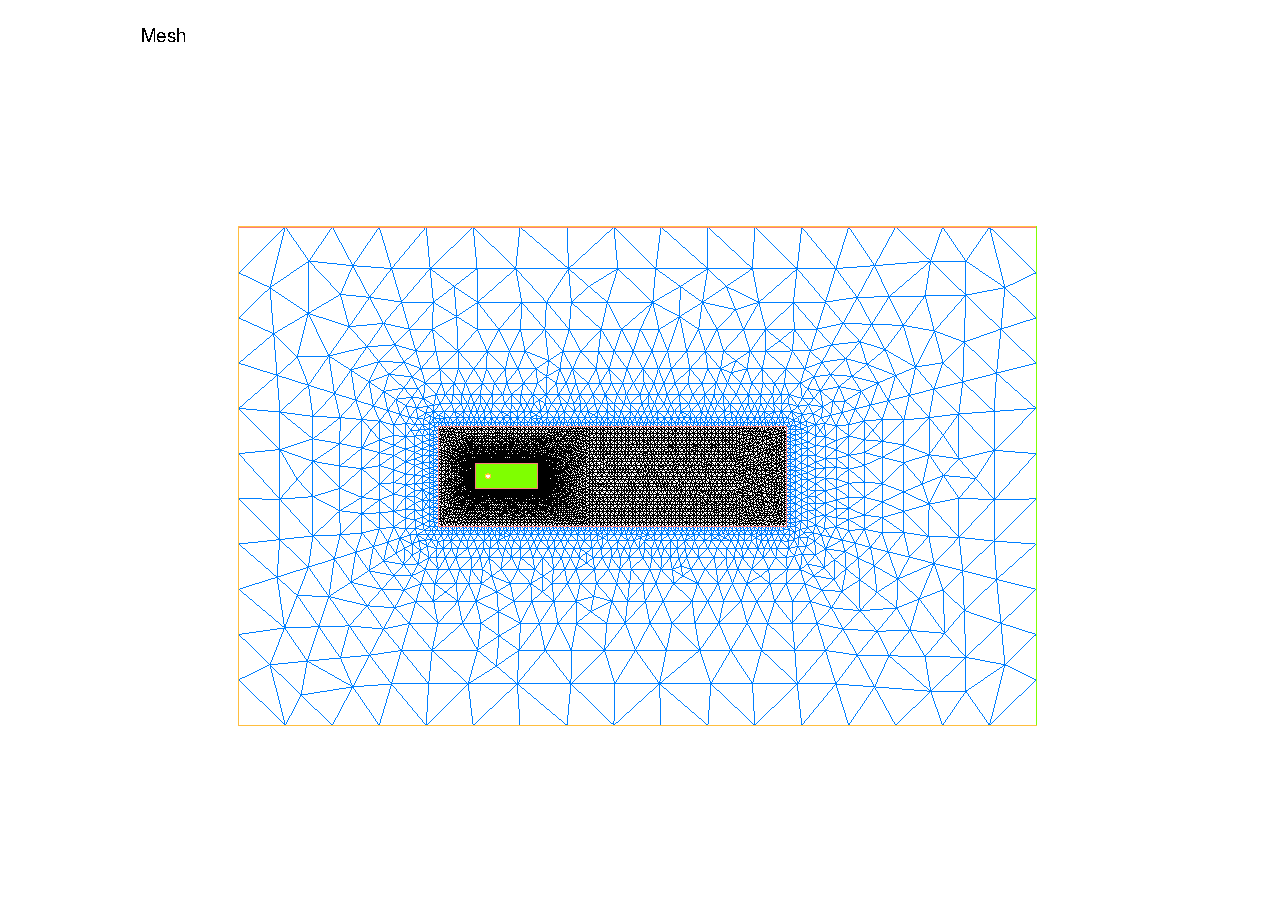
\includegraphics[width = .8 \linewidth]{FIGURES/Mesh.eps}
$$
\caption{Example of computational mesh with dimensions in mapped coordinates and nomenclature of boundaries.} 
\label{fig:Mesh}
\end{figure}




The numerical resolution of the problem was performed with a finite element method,  using the FreeFem++ software. An example of computational mesh, in the $[X,R]$ coordinates, is shown in figure 2. Meshes were generated using Delaunay-Voronoi triangulation of the domain, and subsequently refined locally to fit the steep gradients of both the base flow and the perturbation using the adaptmesh command provided by the Freefem++ software.

For resolution, the Navier-Stokes equations have first to be expressed in terms of the mapped coordinates. For this purpose, the spatial derivatives have to be modified as follows : 

\be
\DP{}{x} \equiv H_x \DP{}{X}  \quad \mbox{ with } H_x =   \frac{1}{G_x'};
\ee
\be
\DP{}{r} \equiv H_r \DP{}{R}  \quad \mbox{ with } H_r =   \frac{1}{G_r'}.
\ee

The incompressible Navier-Stokes operator thus have the following form : 
 
\be
{\cal NS} \left[\begin{array}{c} u_x \\ u_r  \\ p \end{array} \right] =
 \left[\begin{array}{c}
- (u_x  H_x \partial_X u_x + u_r H_r \partial_R u_x) - H_x \partial_X p 
+ \nu \left[ H_x \partial_X ( H_x \partial_X u_x ) + H_r/r\partial_R ( r H_r \partial_r u_x ) \right]
\\
- (u_x  H_x \partial_X u_r + u_r H_r \partial_R u_r) - H_r \partial_R p 
+ \nu \left[ H_x \partial_X ( H_x \partial_X u_r ) - u_r/r^2 + H_r/r\partial_R ( r H_r \partial_r u_r ) \right]
\\
H_x \partial_X u_x + H_r/r \partial_R (r u_r) 
\end{array} \right] 
\label{eq:NS}
\ee

to solve these equations using finite element method, we classically multiply by test functions 
$[u_x^*, u_r^*,p^*]$ and integrate over the domain. Note that this integration has to be done over the physical domain, so in terms of the numerical variables the elementary volume of integration is $dV = r dr dx = (H_x H_r)^{-1} r dR dX$ .
After integration by parts of the pressure gradient and Laplacian terms, we are thus lead to the following weak formulation: 

\be
\begin{array}{l}
\displaystyle
- \int \left[ 
u_x^* \left( u_x  H_x \partial_X u_x + u_r H_r \partial_R u_x \right) 
+ u_r^* \left( u_x  H_x \partial_X u_r + u_r H_r \partial_R u_r \right) 
\right] dV
\\
\displaystyle
+ \int \left[ 
p \left( H_x \partial_X u_x^* + H_r \partial_R u_r^* + u_r^*/r \right) 
-
p^* \left( H_x \partial_X u_x + H_r \partial_R u_r + u_r/r \right) 
\right] dV
\\
\displaystyle
- \int \left[ 
H_x^2 \partial_X u_x \partial_X u_x^* +H_r^2 \partial_R u_x \partial_R u_x^*
\right] dV
\\
\displaystyle
- \int \left[ 
H_x^2 \partial_X u_r \partial_X u_r^* +H_r^2 \partial_R u_r \partial_R u_r^*
+ u_r u_r^*/r^2
\right] dV
\\
= 0.
\end{array}
\ee






Note that with this formulation, the no-traction boundary conditions at the outlet boundary, as well as the symmetry condition at the axis and the zero tangential stress condition at the lateral wall of the cavity are automatically satisfied thanks to the integration by parts. The other boundary conditions are imposed by penalization.

Following a now customary approach, the computation of the base flow is done using a standart Newton method. The algorithm is as follows :
\begin{description}
\item[$(i)$] Start from a guess flow field $[{\bf u}^g;p^g]$.
\item[$(ii)$] Solve the linear system ${\cal NS}[{\bf u}^g,p^g] + {\cal L}_g [\delta {\bf u}, \delta p]$ where $ {\cal L}_g$ is the linearized Navier-Stokes operator around the guess field.
\item[$(iii)$] Obtain a better guess as $ [{\bf u},p] = [{\bf u}^g,p^g] +  [\delta {\bf u}, \delta p]$.
\item[$(iv)$] Repeat until convergence.
\end{description}
The inversion at step $(ii)$ is done with the UMFPACK64 library.

In practice, at point $(i)$ the guess field is generally taken as the base flow computed at a lower value of the Reynolds number. The whole algorithm is thus repeated for increasing values of the Reynolds number to generate a family of base flow. The mesh refinement is applied at each step, so that the refinement, and the number of points of the mesh, increases with the Reynolds number. Note that when using the complex mapping method described above, the radius of convergence of the Newton algorithm seems to be smaller than in the standard case.  This means that the Reynolds number has to be increased moderately between successive base flow computations.

The computation of the perturbations due to harmonic forcing $[u_x',u_r',p']$ is done using the same linear solver UMFPACK64. Note that the structure may involve steeper gradients compared to the base flow. To capture this, the problem is first solved on the refined mesh computed during the base flow computation. The mesh is subsequently refined a second time through the adaptmesh command, and the base flow and the perturbation are finally recomputed on this better mesh. 



%\clearpage

\section{The nonzero thickness case}

We will now consider the case where the jet passes through a hole in a plate with finite thickness, characterized by an aspect ratio $\beta = L/D$. We particularly consider the cases $\beta= 0.3, 0.1 and 1$.



\subsection{Base flows : study of the recirculation region}


\begin{figure}
$$
\begin{array}{cc}
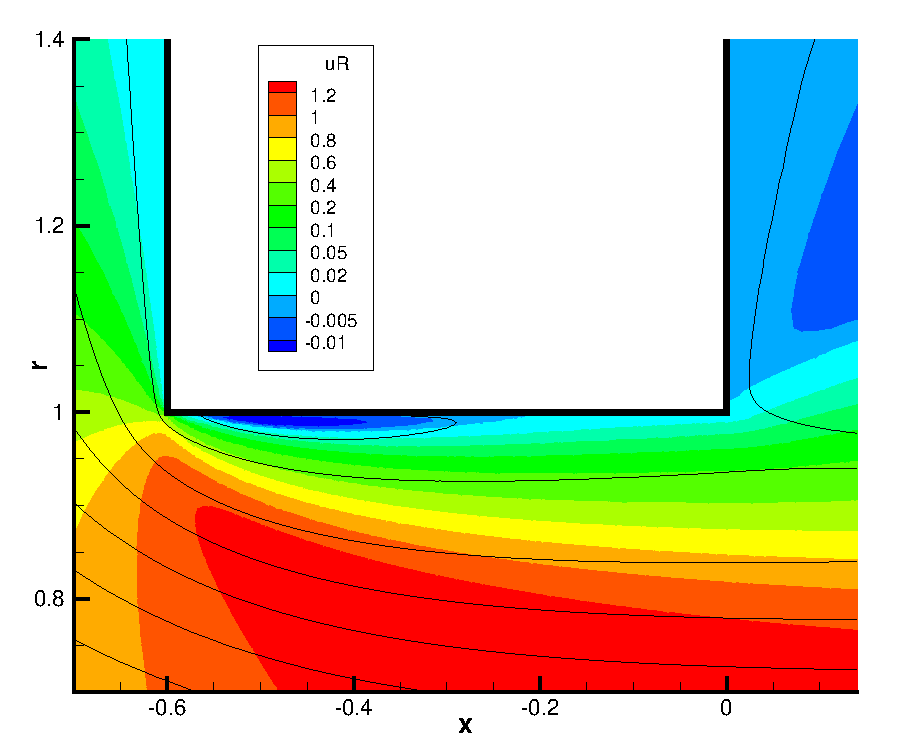
\includegraphics[width=.4\linewidth]{FIGURES/Recirculation_Ep03_Re500.eps} &
\includegraphics[width=.4\linewidth]{FIGURES/Recirculation_Ep03_Re600.eps} \\ 
Re = 500 &  Re = 600 \\
\includegraphics[width=.4\linewidth]{FIGURES/Recirculation_Ep03_Re800.eps} &
\includegraphics[width=.4\linewidth]{FIGURES/Recirculation_Ep03_Re1500.eps} \\
Re = 800 &  Re = 1500
\end{array}
$$
\caption{ Structure of the recirculation region. Colors levels : axial velocity. Black lines : streamfunction.}
\label{fig:Recirc}
\end{figure}

In the case of a hole with finite thickness, the general structure of the flow is similar to the case previously plotted in figure \ref{fig:chbase_C}, with an upstream radially converging flow turning into an almost parallel jet. However, an important feature is the occurence of a recirculation region within the thickness of the hole. This point is illustrated in figure \ref{fig:Recirc} which displays the structure of the flow in the close vicinity of the aperture, for $\beta = 0.3$. For $Re = 500$, the recirculation region takes the form of a narrow bubble trapped close to the upstream corner. As the Reynolds is increased, this bubble expands towards the downstream corner, until it opens up and involves an entraiment of the outer fluid which enters inside the thickness of the plate. Note that for $Re = 800$, the recirculation region still contains a bubble of closed streamlines, but detached from the wall. Further on, this bubble disappears and for $Re = 1500$ the recirculation region is fully open.


\begin{figure}
$$
\includegraphics[width=.7\linewidth]{FIGURES/Recirculation.eps}
$$
\caption{ Intensity of the recirculation flow inside the hole as function of $Re$, 
for $\beta = 0.1$ (dots),  $0.3$ (dashes),  and $1$ (long dashes). }
\label{fig:Umax}
\end{figure}

The intensity of the recirculation region can be characterized by the maximum level of negative velocity within the thickness of the hole, namely $U_{max} = max (-u_{x0})$. This quantity is plotted in figure \ref{fig:Umax} as function of the Reynolds number for $\beta = 0.1, 0.3$ and $1$. It is observed that in all cases, the recirculation region shows up for $Re \approx 400$. The intensity of the recirculation region first grows as the trapped bubble extends to reach the downstream corner, and then decreases as it turns into a fully open one. Not surprisingly, the intensity is larger in the case of a thicker hole, as the bubble is able to extend over a longer region.




\begin{figure}
$$
\includegraphics[width=.7\linewidth]{FIGURES/Alpha_VennaContracta.eps}
$$
\caption{ Vena contracta coefficient as function of $Re$, for $H_h/D_h = 0$ (full line), 
 $H_h/D_h = 0.1$ (dots),  $H_h/D_h = 0.3$ (dashes),  $H_h/D_h = 1$ (long dashes). }
\label{fig:alpha}
\end{figure}

To end up the description of the base flow, we document on figure \ref{fig:alpha} the venna contracta coefficient
deduced from the pressure drop computed from the base flows. It is found that for $Re \approx 10^4$ the venna contracta coefficient reaches a value close to 0.61 in all cases, again in accordance with known experimental results. Note that for the thicker case ($\beta=1$) $\alpha$ is lower than in the other cases for $Re \lesssim 100$, 
meaning that the pressure drop is weaker, but it is maximal for $Re \approx 2000$, a value corresponding approximately to the transition from a closed to an open recirculation region.



%\clearpage
\subsection{Unsteady flow}

\subsubsection{Case $\beta = 0.3$}

%\begin{figure}
%$$
%\includegraphics[width=.4\linewidth]{FIGURES/Cond_Ep03.eps}
%\includegraphics[width=.4\linewidth]{FIGURES/Cond_Ep03Z.eps}
%$$
%\caption{ Real part $\Gamma$ (thick) and Imaginary part $\Delta$ (thin) of the Rayleigh conductivity 
%for a hole of thickness $\beta = 0.3$, for $Re = 100$ ($\cdot \cdot \cdot$), $Re = 500$ (-- --),
%$Re = 800$ (-- $\cdot$ -- ),  $Re = 1500$ (---  ---),  and
%$Re = 3000$ (--- $\cdot$ ---). 
%Plot $(a)$ displays the range $\Omega = [0-5]$, and plot $(b)$ the range $\Omega = [5-15]$ with a different scale for $\gamma$ and $\delta$.}
%\label{fig:Cond03}
%\end{figure}

\begin{figure}
$$
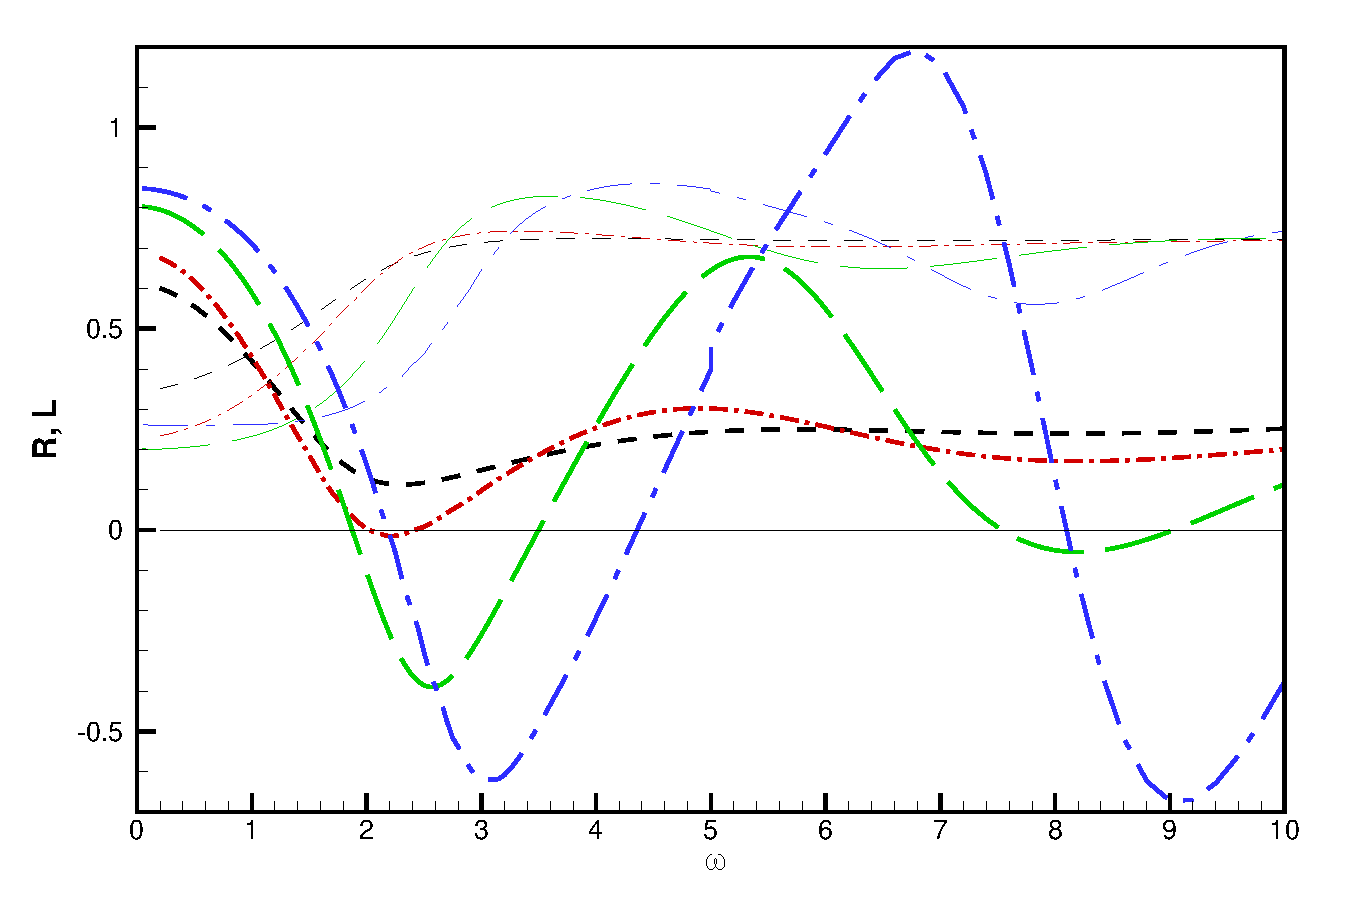
\includegraphics[width=.8\linewidth]{FIGURES/Ep03_RL.eps}
$$
\caption{ Real part $R$ (thick) and Imaginary part $L$ (thin) of the impedance
for a hole of thickness $\beta = 0.3$, for %$Re = 100$ ($\cdot \cdot \cdot$), 
$Re = 500$ (-- --, black),
$Re = 800$ (-- $\cdot$ --, red ),  $Re = 1500$ (---  ---, green),  and
$Re = 3000$ (--- $\cdot$ ---, blue). 
%Plot $(a)$ displays the range $\Omega = [0-5]$, and plot $(b)$ the range $\Omega = [5-15]$ with a different scale for $\gamma$ and $\delta$.
}
\label{fig:Cond03}
\end{figure}


\begin{figure}
$$
\begin{array}{cc}
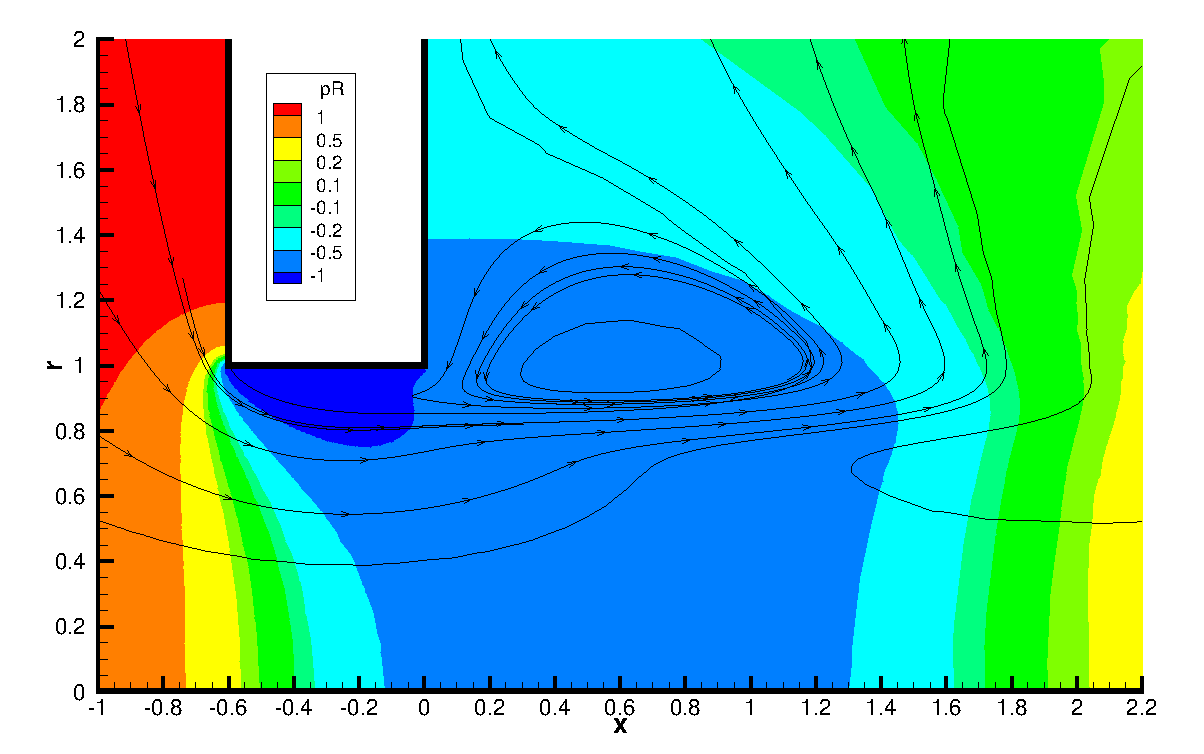
\includegraphics[width=.47\linewidth]{FIGURES/SR_03_1500_1_33.eps} &
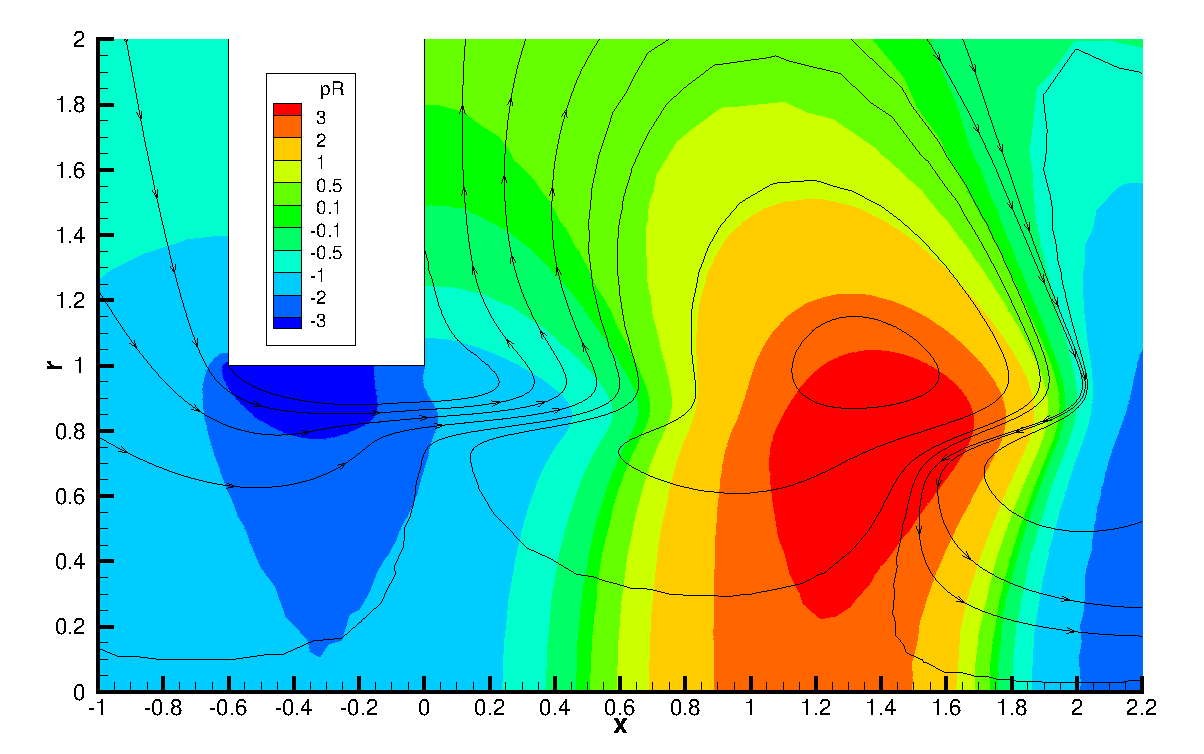
\includegraphics[width=.47\linewidth]{FIGURES/SR_03_1500_2_24.eps} \\
(a) \quad \Omega = 1.33, \, \gamma = 0.799,\, \delta =0.924 & 
(b) \quad \Omega = 2.24,  \, \gamma = 0.904,\, \delta =-0.219 \\
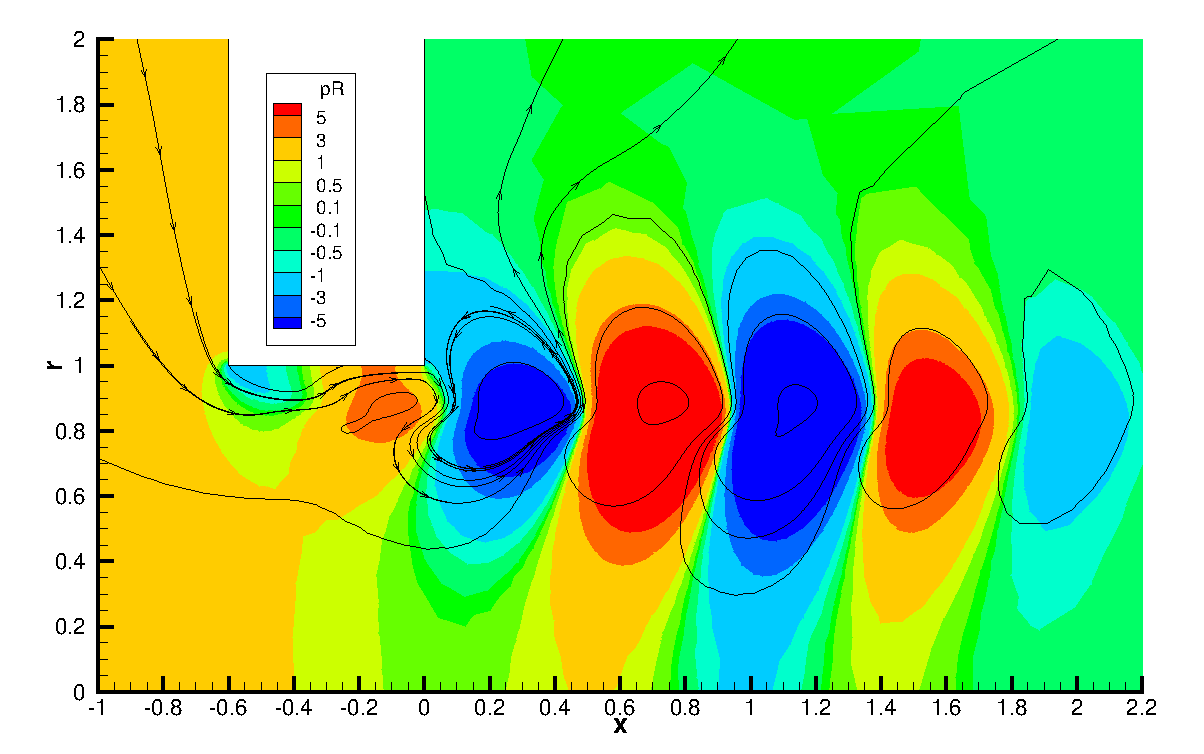
\includegraphics[width=.47\linewidth]{FIGURES/SR_03_1500_5_41.eps} &
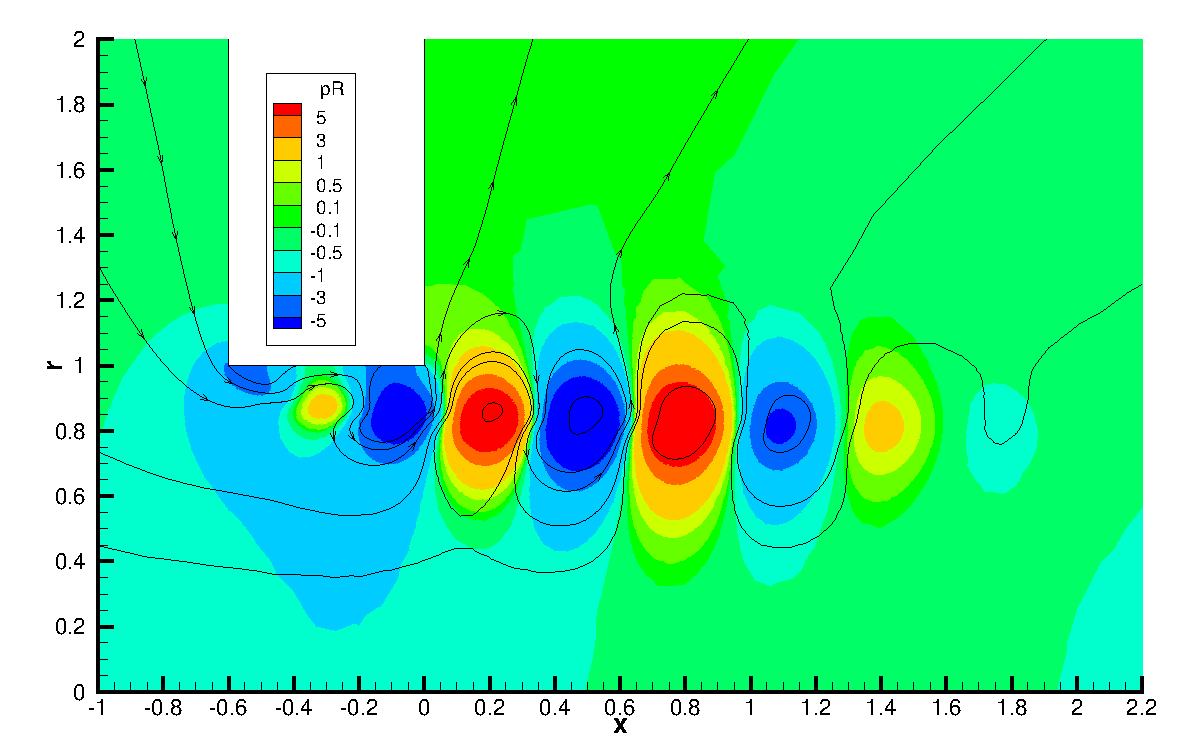
\includegraphics[width=.47\linewidth]{FIGURES/SR_03_1500_8_15.eps} \\
(c) \quad \Omega = 5.41,  \, \gamma = 0.689,\, \delta =0.122 & 
(d) \quad \Omega = 8.15,  \, \gamma = 0.715,\, \delta =-0.0069
\end{array}
$$
\caption{ Structure of the unsteady flow for $\beta = 0.3$ and $Re = 1500$, for different values of $\Omega$.
Real part of the pressure component (color levels) and pseudo-streamlines. 
}
\label{fig:Struct03}
\end{figure}


The most important quantity associated to the unsteady flow is the conductivity $K = 2R (\gamma-i \delta)$. This quantity is plotted as function of the frequency in figure \ref{fig:Cond03} for Reynolds ranging from 500 to 3000.
For $Re = 500$, $\gamma$ and $\delta$ are both positive and are close to the zero-thickness case plotted in figure \ref{fig:Cond0}. For $Re= 800$, one observes that the imaginary part $\delta$ becomes negative for 
$\Omega \approx 2.2$. As explained in section 2, this property is directly related to a possible instability. As the Reynolds number is increased further, one observes that the region of negative $\delta$ gets larger and reaches larger values. Note also that the negative, minimum value of $\delta$ is associated to a maximum of the real part $\gamma$. 
Figure \ref{fig:Cond03}$(b)$ magnifies the range $\Omega = [5-15]$ and shows that a second region of instability shows up for $Re \gtrsim 1500$, with higher frequencies in the range $\Omega \approx 9$. This is again associated with a maximum of the real part $\gamma$.

To explain these trends, and in particular the possibility for negative $\delta$, we detail the structure of the flow perturbation for four values the frequency, corresponding respectively to two positive maxima ($a$ and $c$)
 and two negative minima  ($b$ and $d$) of $\delta$. We recall that these structure are computed with the complex mapping method, so the details are not significant for $x \gtrsim 2$. However, several significant points can be noted. First, it is clear that in the unstable cases ($b$ and $d$) the pressure levels are negative in the upstream region, while they are positive in the stable cases ($a$ and $c$). Recalling that the pressure level far away in the downstream region is set to zero, this means that in the unstable cases the fluctuating flow goes against the pressure gradient. A second salient feature can be noted when looking at the streamlines in the vicinity
 of the lower corner. In the unstable cases ($b$ and $d$) the fluctuating flow emerging from the hole goes up along the outer wall, although in the stable cases stable cases ($a$ and $c$) the opposite happens, meaning that the fluid coming from along the wall is entrained within the jet.


\subsubsection{Case $\beta = 1$}

%\begin{figure}
%$$
%\begin{array}{cc}
%\includegraphics[width=.4\linewidth]{FIGURES/Cond_Ep1.eps}
%\includegraphics[width=.4\linewidth]{FIGURES/Z_Ep1.eps}
%\end{array}
%$$
%\caption{ Conductivity and impedance for a hole with thickness $\beta = 1$ :  
%$(a)$ Real part $\gamma$ (thick) and Imaginary part $\delta$ (thin) of the Rayleigh conductivity for 
%$Re = 500$ (-- --), $Re = 800$ (--$\cdot$--), $Re = 1200$ ( --$ \cdot \cdot$-- ).
%$(b)$ Real (thick) and Imaginary (thin)  parts  of the Impedance for $Re = 1500$ (---  ---)
%and  $Re = 3000$ (---$\cdot$---).
%}
%\label{fig:Cond1}
%\end{figure}

\begin{figure}
$$
\begin{array}{cc}
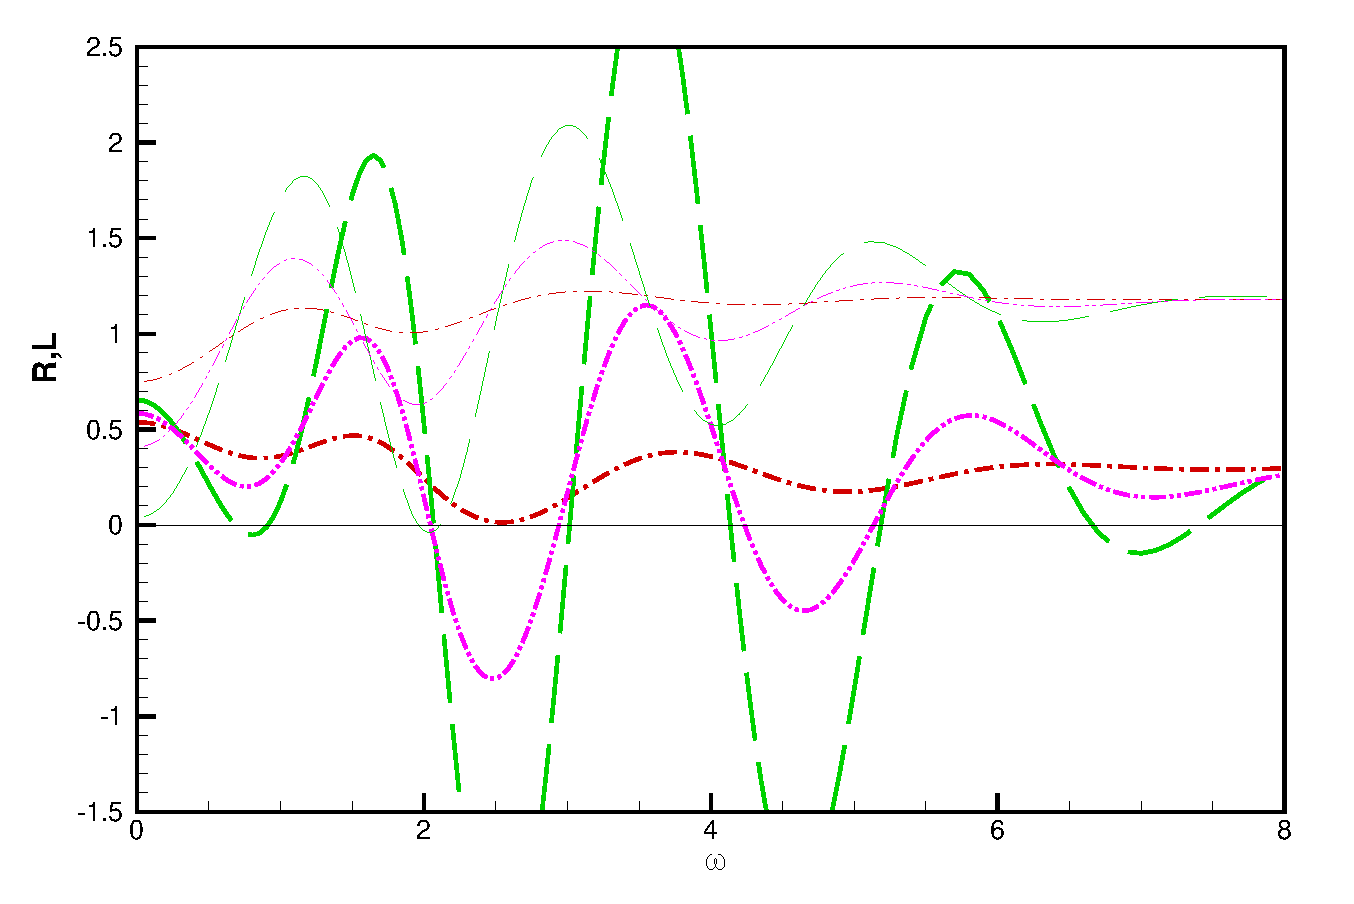
\includegraphics[width=.8\linewidth]{FIGURES/Ep1_RL.eps}
\end{array}
$$
\caption{ 
$(a)$ Real part $R$ (thick) and Imaginary part $L$ (thin) of the impedance for a hole of thickness
$\beta = 1$, for $Re = 800$ (--$\cdot$--, red), $Re = 1200$ ( --$ \cdot \cdot$--, magenta) and $Re = 1500$ (---  ---, green).
}
\label{fig:Cond1}
\end{figure}

We now consider the case of a thicker hole with aspect ratio $\beta = 1$. Figure \ref{fig:Cond1}$(a)$ plots the conductivity for $Re$ from 500 to 1200. As in the previous case, one can see the existence of several frequency intervals where the imaginary part $\delta$ becomes negative. For instance, for $Re = 800$ this occurs for $\Omega \approx 2.5$ while for $Re = 1200$ there are two intervals around 2.1 and 4.5. One can also notice that the real part $\gamma$ experiences much larger oscillations than in the previous case. 

As the Reynolds number is increased, both real and imaginary parts of the conductivity reach very large value, so it becomes more appropriate to plot the impedance $Z_{app} = -i \omega/K$ instead of the conductivity. Figure \ref{fig:Cond1}$(b)$ plots this quantity as function of the frequency for $Re = 1500$ and $3000$.
Recall that the criterion $\delta<0$ leading to possible instability is equivalent to $Z_r<0$, which occurs in at least three intervals in the range of frequencies considered. Another important result which can be seen in this figure is the existence of true zeros of the impedance. This happens in particular for $Re = 1500$ at $\Omega \approx 2.07$. This property indicates the existence of a linear perturbation with nonzero flow rate but zero pressure jump across the aperture. So, the jet may be subject to self-sustained oscillation even in the absence of an acoustic resonator located upstream. This indicates the possibility of a purely hydrodynamical instability. This fact will be confirmed in section 6.









\begin{figure}
$$
\begin{array}{cc}
\includegraphics[width=.47\linewidth]{FIGURES/SR_1_1200_2_25.eps} &
\includegraphics[width=.47\linewidth]{FIGURES/SR_1_1200_4_55.eps} \\
(a) \quad Re = 1200, \, \Omega = 2.25, \, \gamma = 0.544,\, \delta =-0.161 & 
(b) \quad Re = 1200, \, \Omega = 4.45,  \, \gamma = 0.0.449,\, \delta =-0.038 \\
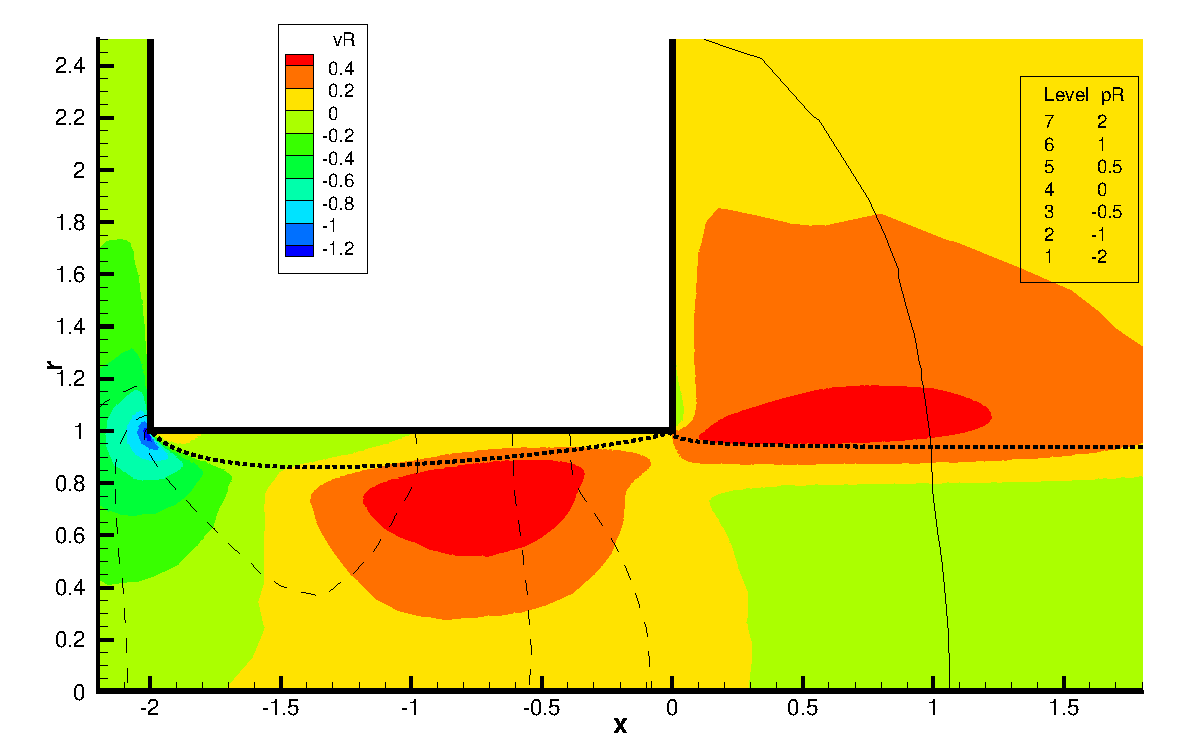
\includegraphics[width=.47\linewidth]{FIGURES/SR_1_1500_08.eps} &
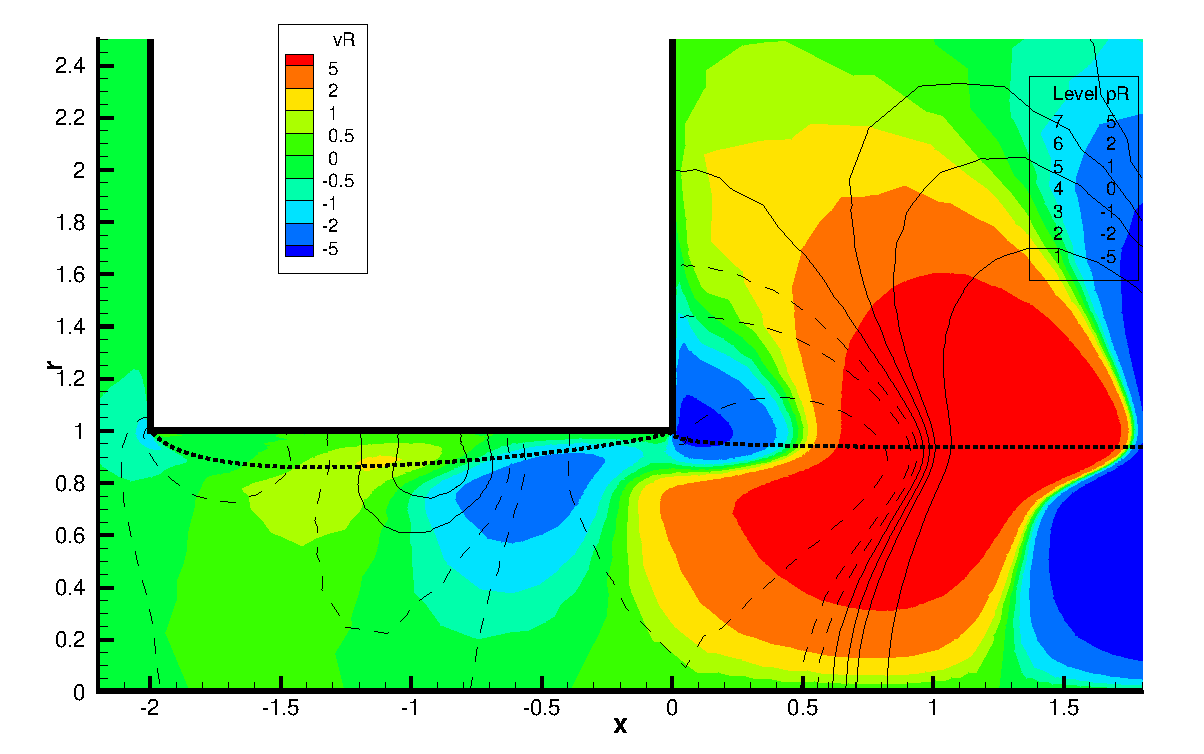
\includegraphics[width=.47\linewidth]{FIGURES/SR_1_1500_2_07.eps} \\
(c) \quad Re = 1500, \, \Omega = 0.8,  \, \gamma = 0.380,\, \delta =-0.019 & 
(d) \quad Re = 1500, \, \Omega = 2.07,  \, \gamma = -15.637,\, \delta =-6.099
\end{array}
$$
\caption{ Structure of the unsteady flow for $\beta = 0.3$ and $Re = 1500$, for different values of $\Omega$.
The color levels indicate the real part of the radial velocity components, while the thin lines indicate the real part of the pressure component (dashed for negative levels). The thick dotted line indicate the recirculation region. 
Plot $(d)$ corresponds to the minimum impedance for $Re=1500$, namely $Z = -0.0224+0.0574i$.
}
\label{fig:Struct1}
\end{figure}


Finally, figure \ref{fig:Struct1} depicts the structure of the oscillating flow for the two first minima of $\delta$ for $Re = 1200$ (plots $a$ and $b$). One can observe that these perturbations display respectively 4 and 6 structures within the thickness of the hole. Note that a minimum of $\delta$ also exists for $Re =1200$ at $\Omega \approx 1$, but the value of $\delta$ remains positive. For $Re= 1500$, this first minimum becomes negative, and the
corresponding structure is plotted in figure \ref{fig:Struct1}$(c)$. As expected, it displays only two vortical structures within the thickness of the hole. Finally, figure \ref{fig:Struct1}$(d)$ displays the case corresponding to the minimum of $|Z_{app}|$ for $Re = 1500$. 
The structure is much similar to the case plotted in \ref{fig:Struct1}$(a)$, not surprisingly because the frequency is close.






\subsubsection{Case $\beta = 0.1$}


%\begin{figure}
%$$
%\includegraphics[width=.4\linewidth]{FIGURES/Cond_Ep01.eps}
%\includegraphics[width=.4\linewidth]{FIGURES/Cond_Ep01Z.eps}
%$$
%\caption{ Real part $\Gamma$ (thick) and Imaginary part $\Delta$ (thin) of the Rayleigh conductivity 
%for a hole of thickness $\beta = 0.1$, for $Re = 500$ (-- --),
%$Re = 800$ ($\cdot$ -- $\cdot$), $Re = 1500$ (---  ---), $Re = 3000$ (------).
%The right plot displays $\Delta$ in the range $5< \Omega < 15$, with a magnified scale allowing to show the region where it becomes negative.
%NB THE CASES WITH RE = 4500 ARE SPURIOUS.
%}
%\label{fig:Cond01}
%\end{figure}


\begin{figure}
$$
\includegraphics[width=.8\linewidth]{FIGURES/Ep01_RL.eps}
$$
\caption{ Real part $R$ (thick) and Imaginary part $L$ (thin) of the impedance
for a hole of thickness $\beta = 0.1$, for $Re = 800$ ($\cdot$ -- $\cdot$), 
$Re = 1500$ (---  ---), $Re = 3000$ (--- - ---).
}
\label{fig:Cond01}
\end{figure}



As a third case, we consider a thinner plate with $\beta = 0.1$. The conductivities are plotted in figure 
\ref{fig:Cond01}. We note that a negative minimum of $\delta$ is also observed but it only occurs for 
$Re \gtrsim 3000$ and at larger frequencies than in the previous cases, namely $\Omega = 8.2$.

Comparing the three previous cases, it is interesting to note that the minimum frequency where an negative $\delta$ can occur is inversely proportional to the thickness. Indeed, defining the Strouhal number based on the thickness
leads to $St = L \omega /U_M \approx 1 $  in the three cases. 
Note that the fact that the frequency of the whistling tone is inversely proportional to the thickness was already noted by Bouasse.


\subsubsection{Case of a rounded hole}




\begin{figure}
$$
\includegraphics[width=.7\linewidth]{FIGURES/CBRounded_3000_Complex.eps}
$$
\caption{Base flow for a rounded hole of thickness $\beta = 0.3$, with $Re = 3000$ 
(in numerical coordinates $(X,R)$, with complex mapping). 
}
\label{fig:chbase_C}
\end{figure}



The previous cases indicate that the source of instability is linked to the existence of a recirculation region, and this feature is particularly favored by the existence of sharp corners upstream and downstream of the hole. To support this statement, we investigated the case of a rounded hole. The aspect ratio is taken as $\beta=0.3$, but 
the shape of the hole is taken as a semicircle. Figure \ref{fig:chbase_C} displays the structure of the base flow in this case, with $Re = 3000$. It can be noted that the flow effectively detaches from the wall while passing through the hole leading to an open recirculation region. However, this recirculation region is much weaker than that observed in the case of a hole with sharp edge. Clearly, the absence of a sharp corner leads to a much smoother recirculation region, and therefore much less potential for instability.


\begin{figure}
$$
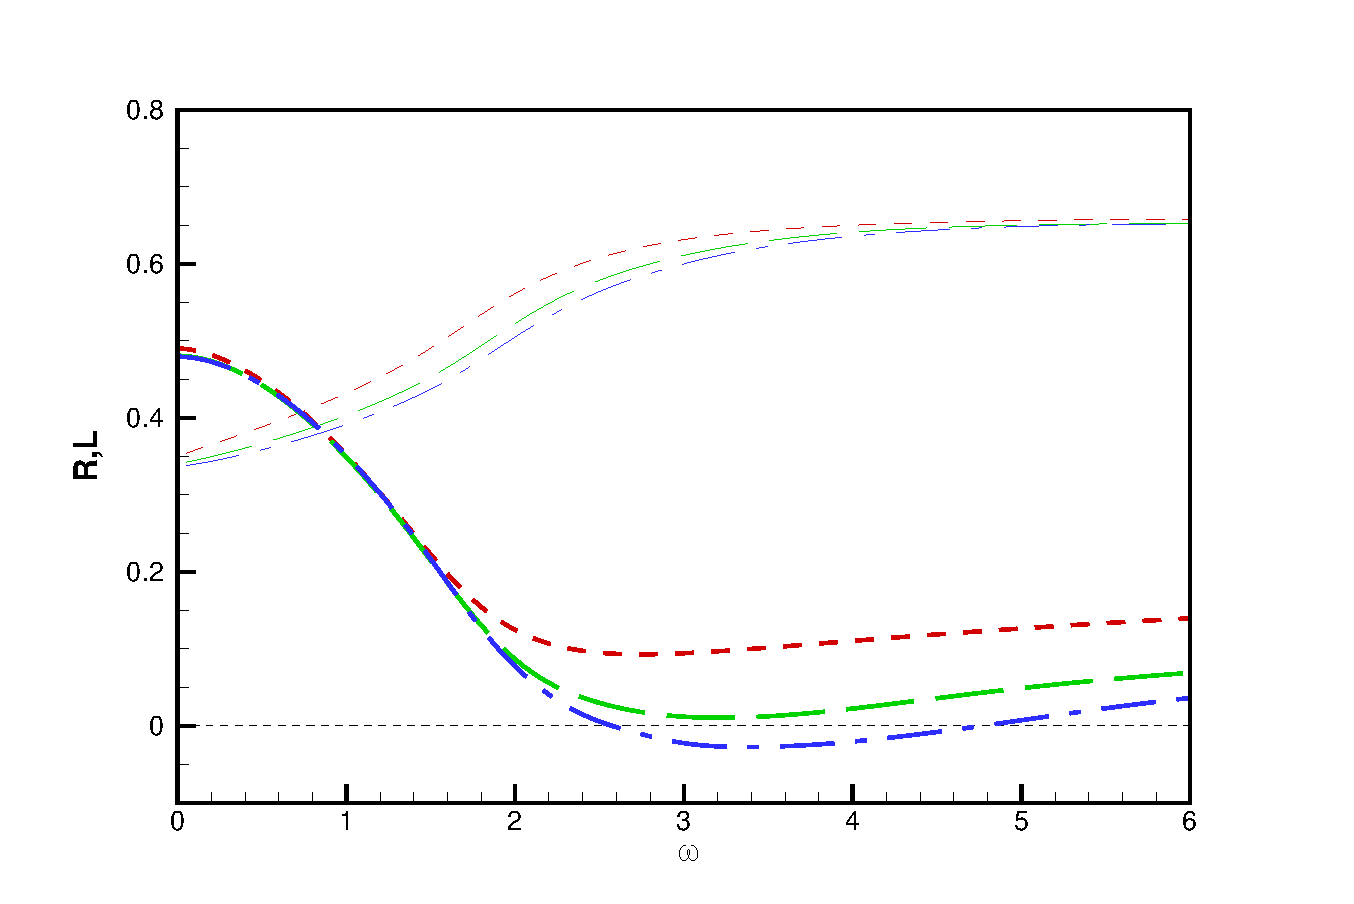
\includegraphics[width=.7\linewidth]{FIGURES/Rounded_RL.eps}
$$
\caption{ Real part $R$ (thick) and Imaginary part $L$ (thin) of the impedance 
for a rounded hole with thickness $\beta=0.3$, with
$Re = 500$ ($\cdot$ -- $\cdot$), $Re = 1500$ (---  ---), $Re = 3000$ (--- - ---).
Plot $(b)$ is a magnification of the range where $\delta$ becomes negative.
}
\label{fig:CondR}
\end{figure}

Figure \ref{fig:CondR} displays the conductivity for the case of a rounded hole, and suppports this conclusion. Indeed, a negative minimum of $\delta$ is effectively observed for $\Omega \approx 3$, which is about in the same range than for the sharp corner with the same aspect ratio, but this happens at much larger values of the Reynolds number, namely $Re = 3000$.



\section{Parametric study}

\begin{figure}
$$
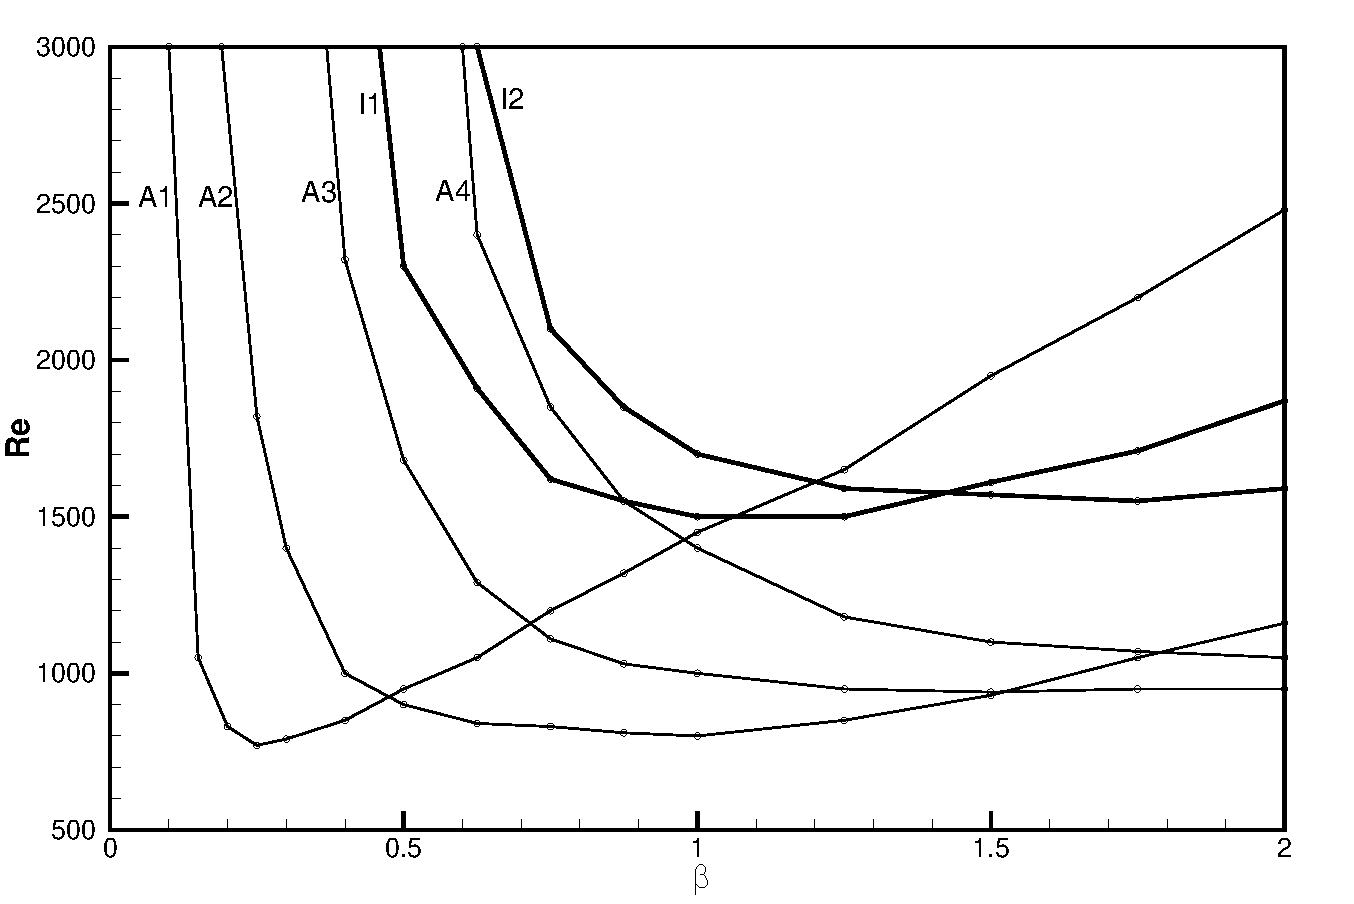
\includegraphics[width=.7\linewidth]{FIGURES/Seuils_Re.eps}
$$
\caption{ Thresholds for the onset of acoustic instability (A1 to A4) and of hydrodynamical instability (I1 and I2).
}
\label{fig:ThresholdsRe}
\end{figure}

\begin{figure}
$$
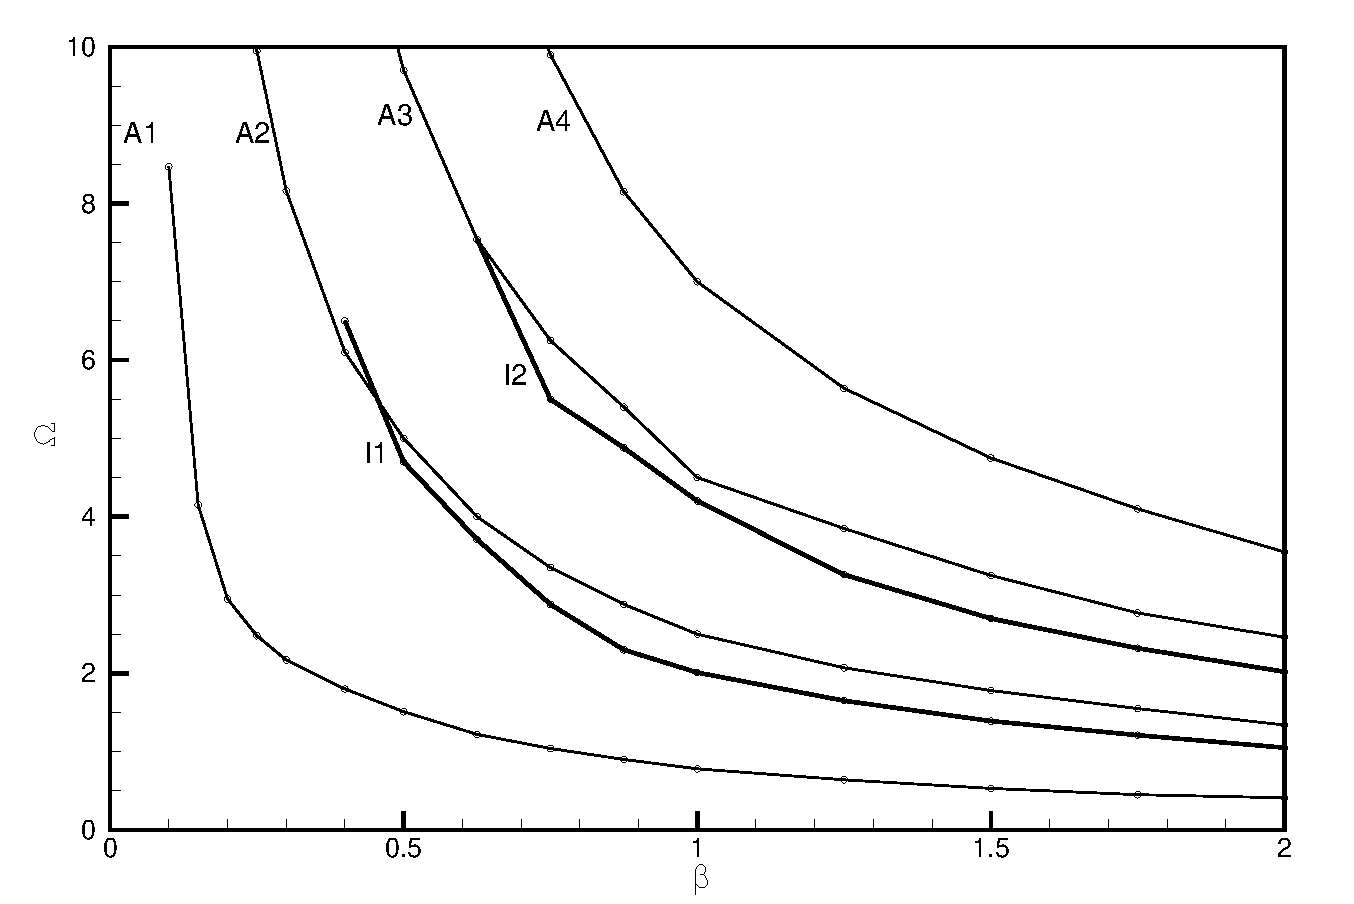
\includegraphics[width=.7\linewidth]{FIGURES/Seuils_Om.eps}
$$
\caption{ Frequencies corresponding to acoustic instability (A1 to A4) and of hydrodynamical instability (I1 and I2).
}
\label{fig:ThresholdsRe}
\end{figure}


\section{Conclusions}


\appendix
\section{Numerical validations}
Only the mesh and mayle the parameter $L_M$


%%%%%%%%%%%%%%%%%%%%%%%%%%%%%%%%%

\bibliographystyle{jfm}

\bibliography{OneHole_PartII_zerothickness}


\end{document}